\documentclass{article}
\usepackage[letterpaper,top=2cm,bottom=2cm,left=3cm,right=3cm,marginparwidth=1.75cm]{geometry}
\usepackage[russian]{babel}
\usepackage{amsmath}
\usepackage{graphicx}
\usepackage[utf8]{inputenc}
\usepackage[colorlinks=true, allcolors=blue]{hyperref}
\usepackage[pdf]{graphviz}
\graphicspath{ {./static/1/}{./static/2/}{./static/3/}{./static/4/}}
\usepackage{ucs} 

\title{ТМВ Домашнее задание №1}
\author{А-13б-19 Головин Антон}
\date{5 апреля 2022}

\begin{document}
\maketitle

%%%%%%%%%%%%%%%%%%%%%%%%%%%%%%%%%%%%%%%%%%% Задание 1 %%%%%%%%%%%%%%%%%%%%%%%%%%%%%%%%%%%%%%%%%%%
\section{Задание №1. Построить конечный автомат, распознающий язык.}
\begin{enumerate}
%%%%%%%%%%%%%%% 1.1 %%%%%%%%%%%%%%%
\\
\item {$L = \{ w \in \{a,b,c\}^* \mid |w|_c = 1 \} $} \\
    \begin{center}
        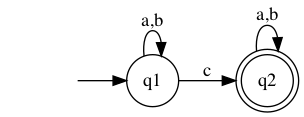
\includegraphics[width=0.4\textwidth]{g11.png}
    \end{center}

%%%%%%%%%%%%%%% 1.2 %%%%%%%%%%%%%%%
\item {$L = \{ w \in \{a,b\}^*  \mid  |w|_a \le 2, {|w|_b} \ge 2 \}$} \\ \\
    Это задача на прямое произведение. \\ \\
    $L_{11} = \{ w \in \{a,b\}^*  \mid  |w|_a \le 2 \} $\\
    \begin{center}
        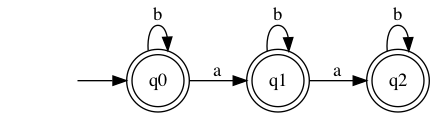
\includegraphics[width=0.5\textwidth]{g121.png}
    \end{center}

    $L_{12} = \{ w \in \{a,b\}^*  \mid  |w|_b \ge 2 \} $
    \begin{center}
        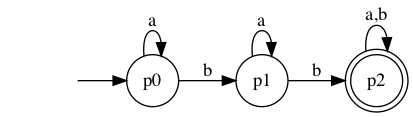
\includegraphics[width=0.5\textwidth]{g122.png}
    \end{center}
    
    \newpage
    
    \begin{center}
    \[
        L = L_{11} \times L_{12} \Rightarrow \\
        A_1 = \left\langle \sum_{1}, Q_1, S_1, T_1, \delta_1\right\rangle \quad 
        A_2 = \left\langle \sum_{2}, Q_2, S_2, T_2, \delta_2\right\rangle
    \]
    
    \[
        \sum = \{a, b\} \\
        Q = Q_1 \times Q_2 = \{q0p0, q0p1, q0p2, q1p0, q1p1, q1p2, q2p0, q2p1, q2p2\} \\
        S = \left\langle S_1, S_2\right\rangle = \left\langle q0,p0 \right\rangle \\
        T = T_1 \times T_2 = \left\langle q2p2, q1p2, q0p2 \right\rangle
    \]
    
    $$\delta(\left\langle q1,q2 \right\rangle, c) = \left\langle \delta_1(q_1, c), \delta_2(q_2, c)\right\rangle $$

    \begin{tabular}{ |c|c|c| } 
        \hline
        &$\textbf{a}$ & $\textbf{b}$ \\
        \hline
        \left\langle q0,p0 \right\rangle & \left\langle q1,p0 \right\rangle & \left\langle q0,p1 \right\rangle \\
        \hline
        \left\langle q0,p1 \right\rangle & \left\langle q1,p1 \right\rangle & \left\langle q0,p2 \right\rangle \\
        \hline
        \left\langle q0,p2 \right\rangle & \left\langle q1,p2 \right\rangle & \left\langle q0,p2 \right\rangle \\
        \hline
        \left\langle q1,p0 \right\rangle & \left\langle q2,p0 \right\rangle & \left\langle q1,p0 \right\rangle \\
        \hline
        \left\langle q1,p1 \right\rangle & \left\langle q2,p1 \right\rangle & \left\langle q1,p2 \right\rangle \\
        \hline
        \left\langle q1,p2 \right\rangle & \left\langle q2,p2 \right\rangle & \left\langle q1,p2 \right\rangle \\
        \hline
        \left\langle q2,p0 \right\rangle &  -  & \left\langle q2,p1 \right\rangle \\
        \hline
        \left\langle q2,p1 \right\rangle &  -  & \left\langle q2,p2 \right\rangle \\
        \hline
        \left\langle q2,p2 \right\rangle &  -  & \left\langle q2,p2 \right\rangle \\
        \hline
    \end{tabular}
    \end{center}
    
    \begin{center}
        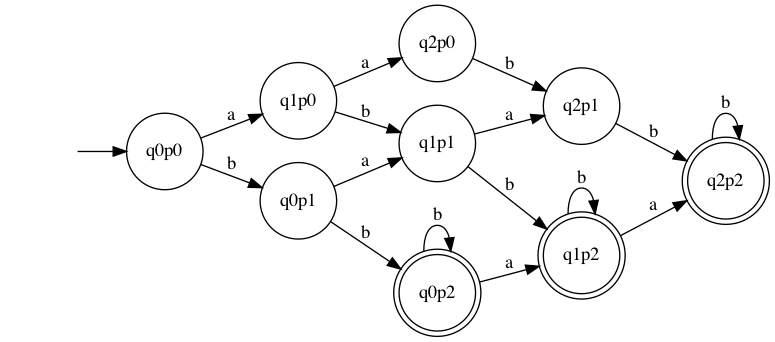
\includegraphics[width=0.8\textwidth]{g12.png}
    \end{center}
 
%%%%%%%%%%%%%%% 1.3 %%%%%%%%%%%%%%%
\item {$L_3 = \{ w \in \{a,b\}^*  \mid  |w|_a \neq |w|_b \} $} \\ \\
    Конечный автомат нельзя построить, потому что требуется сравнивать количество символов $\Rightarrow$ нерегулярный язык.

%%%%%%%%%%%%%%% 1.4 %%%%%%%%%%%%%%%
\item {$L = \{ w \in \{a,b\}^*  \mid  w w = w w w \}$} \\ \\
    Язык, допускающий пустое слово.
    \begin{center}
        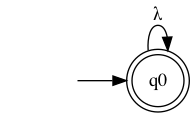
\includegraphics[width=0.3\textwidth]{g14.png}
    \end{center}
\end{enumerate}




%%%%%%%%%%%%%%%%%%%%%%%%%%%%%%%%%%%%%%%%%%% Задание 2 %%%%%%%%%%%%%%%%%%%%%%%%%%%%%%%%%%%%%%%%%%%
\section{Задание №2. Построить конечный автомат, используя прямое произведение.}
\begin{enumerate}
%%%%%%%%%%%%%%% 2.1 %%%%%%%%%%%%%%%
\\
\item {$L_1 = \{ w \in \{a,b\}^*   \mid  |w|_a \ge 2  \wedge   |w|_b \ge 2 \} \\ $} \\
    $L_{11} = \{ w \in \{a,b\}^*   \mid   |w|_a \ge 2 \} \\$
    \begin{center}
        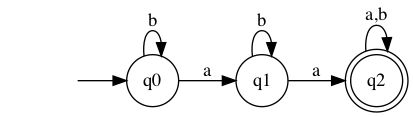
\includegraphics[width=0.5\textwidth]{g211.png}
    \end{center}

    $L_{12} = \{ w \in \{a,b\}^*   \mid   |w|_b \ge 2 \} \\$
    \begin{center}
        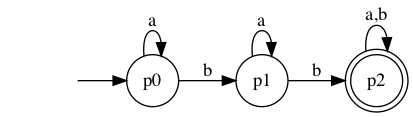
\includegraphics[width=0.5\textwidth]{g212.png}
    \end{center}
    
    \begin{center}
    \[
        L_1 = L_{11} \times L_{12} \Rightarrow \\
        A_1 = \left\langle \sum_{1} , Q_1, S_1, T_1, \delta_1\right\rangle \quad 
        A_2 = \left\langle \sum_{2}, Q_2, S_2, T_2, \delta_2\right\rangle
    \]
    
    \[
        \sum = \{a, b\} \\
        Q = Q_1 \times Q_2 = \{q0p0, q0p1, q0p2, q1p0, q1p1, q1p2, q2p0, q2p1, q2p2\} \\
        S = \left\langle S_1, S_2 \right\rangle = \left\langle q0,p0 \right\rangle \\
        T = T_1 \times T_2 = \left\langle q2p2, q1p2, q0p2 \right\rangle
    \]
    \end{center}
    
    
    
    \begin{center}
    \begin{tabular}{ |c|c|c| } 
        \hline
        & $\textbf{a}$ & $\textbf{b}$ \\
        \hline
        \left\langle q0,p0 \right\rangle & \left\langle q1,p0 \right\rangle & \left\langle q0,p1 \right\rangle \\
        \hline
        \left\langle q0,p1 \right\rangle & \left\langle q1,p1 \right\rangle & \left\langle q0,p2 \right\rangle \\
        \hline
        \left\langle q0,p2 \right\rangle & \left\langle q1,p2 \right\rangle & \left\langle q0,p2 \right\rangle \\
        \hline
        \left\langle q1,p0 \right\rangle & \left\langle q2,p0 \right\rangle & \left\langle q1,p1 \right\rangle \\
        \hline
        \left\langle q1,p1 \right\rangle & \left\langle q2,p1 \right\rangle & \left\langle q1,p2 \right\rangle \\
        \hline
        \left\langle q1,p2 \right\rangle & \left\langle q2,p2 \right\rangle & \left\langle q1,p2 \right\rangle \\
        \hline
        \left\langle q2,p0 \right\rangle & \left\langle q2,p0 \right\rangle & \left\langle q2,p1 \right\rangle \\
        \hline
        \left\langle q2,p1 \right\rangle & \left\langle q2,p1 \right\rangle & \left\langle q2,p2 \right\rangle \\
        \hline
        (q2,p2) & (q2,p2) & (q2,p2) \\
        \hline
    \end{tabular}
    \end{center}
    
    \begin{center}
        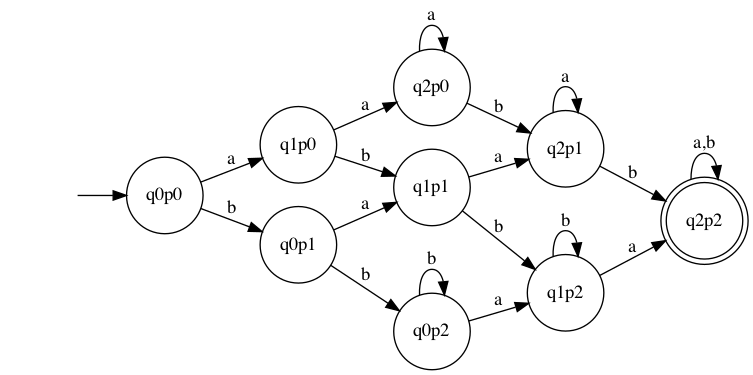
\includegraphics[width=0.8\textwidth]{g21.png}
    \end{center}
    
%%%%%%%%%%%%%%% 2.2 %%%%%%%%%%%%%%%
\item {$L_2 = \{ w \in \{a,b\}^*   \mid   |w| \ge 3 \wedge |w| \text{ нечётное}\} $} \\ \\
    $L_{21} = \{ w \in \{a,b\}^*   \mid  |w| \ge 3 \} \\$
    \begin{center}
        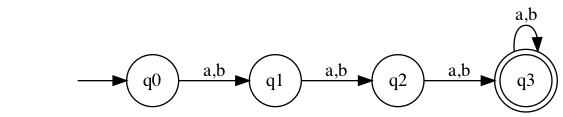
\includegraphics[width=0.8\textwidth]{g221.png}
    \end{center}
    
    $L_{22} = \{ w \in \{a,b\}^*   \mid   |w| \text{ нечётное}\} \\$
    \begin{center}
        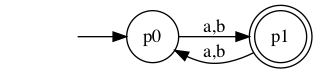
\includegraphics[width=0.5\textwidth]{g222.png}
    \end{center}
    
    \begin{center}
    \[
        L_2 = L_{21} \times L_{22} \Rightarrow \\
        A_1 = \left\langle\sum_{1} , Q_1, S_1, T_1, \delta_1\right\rangle \quad 
        A_2 = \left\langle\sum_{2}, Q_2, S_2, T_2, \delta_2\right\rangle
    \]
    
    \[
        \sum = \{a, b\} \\
        Q = \{q0p0, q0p1, q1p0, q1p1, q2p0, q2p1, q3p0, q3p1\} \\
        S = \left\langle q0,p0 \right\rangle \\
        T = \left\langle q3,p1 \right\rangle \\
    \]
    
    
    
    
    \begin{tabular}{ |c|c|c| } 
        \hline
        & $\textbf{a}$ & $\textbf{b}$ \\
        \hline
        \left\langle q0,p0 \right\rangle & \left\langle q1,p1 \right\rangle & \left\langle q1,p1 \right\rangle \\
        \hline
        \left\langle q0,p1 \right\rangle & \left\langle q1,p0 \right\rangle & \left\langle q1,p0 \right\rangle \\
        \hline
        \left\langle q1,p0 \right\rangle & \left\langle q2,p1 \right\rangle & \left\langle q2,p1 \right\rangle \\
        \hline
        \left\langle q1,p1 \right\rangle & \left\langle q2,p0 \right\rangle & \left\langle q2,p0 \right\rangle \\
        \hline
        \left\langle q2,p0 \right\rangle & \left\langle q3,p1 \right\rangle & \left\langle q3,p1 \right\rangle \\
        \hline
        \left\langle q2,p1 \right\rangle & \left\langle q3,p0 \right\rangle & \left\langle q3,p0 \right\rangle \\
        \hline
        \left\langle q3,p0 \right\rangle &  \left\langle q3p,1 \right\rangle & \left\langle q3,p1 \right\rangle \\
        \hline
        \left\langle q3,p1 \right\rangle &  \left\langle q3,p0 \right\rangle & \left\langle q3,p0 \right\rangle \\
        \hline
    \end{tabular}
    \end{center}
    \begin{center}
        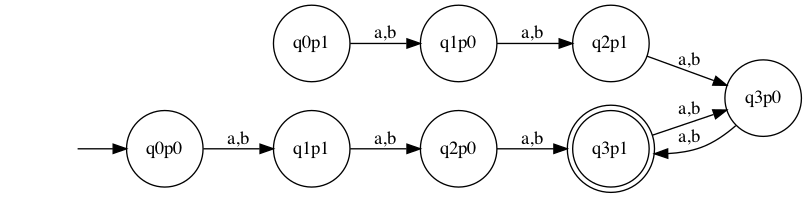
\includegraphics[width=0.8\textwidth]{g22.png}
    \end{center}
    Упрощаем (для 2.5):
    \begin{center}
        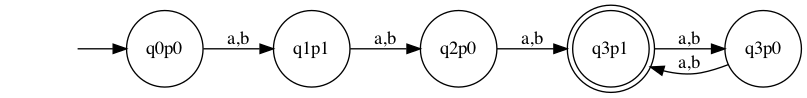
\includegraphics[width=0.8\textwidth]{g22_easy.png}
    \end{center}

%%%%%%%%%%%%%%% 2.3 %%%%%%%%%%%%%%%
\item {$L_3 = \{w \in \{a,b\}^*   \mid   |w|_a \text{ чётно} \wedge |w|_b \text{ кратно трём} \} $} \\ \\
    $L_{31} = \{w \in \{a,b\}^*   \mid   |w|_a \text{ чётно} \} $\\
    \begin{center}
        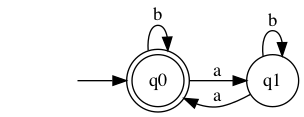
\includegraphics[width=0.4\textwidth]{g231.png}
    \end{center}
    $L_{32} = \{w \in \{a,b\}^*   \mid   |w|_b \text{ кратно трём} \} $\\
    \begin{center}
        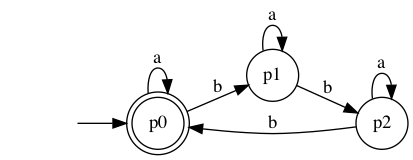
\includegraphics[width=0.5\textwidth]{g232.png}
    \end{center}
    
    \begin{center}
    \[
        L_3 = L_{31} \times L_{32} \Rightarrow \\
        A_1 = \left\langle \sum_{1} , Q_1, S_1, T_1, \delta_1\right\rangle \quad 
        A_2 = \left\langle \sum_{2}, Q_2, S_2, T_2, \delta_2\right\rangle
    \]
    
    \[
        \sum = \{a, b\} \\
        Q = \{q0p0, q0p1, q0p2, q1p0, q1p1, q1p2\} \\
        S = \left\langle q0,p0 \right\rangle \\
        T = \left\langle q0,p0 \right\rangle \\
    \]
    
    \begin{tabular}{ |c|c|c| } 
        \hline
        & $a$ & $b$ \\
        \hline
        \left\langle q0,p0 \right\rangle & \left\langle q1,p0 \right\rangle & \left\langle q0,p1 \right\rangle \\
        \hline
        \left\langle q0,p1 \right\rangle & \left\langle q1,p1 \right\rangle & \left\langle q0,p2 \right\rangle \\
        \hline
        \left\langle q0,p2 \right\rangle & \left\langle q1,p2 \right\rangle & \left\langle q0,p0 \right\rangle \\
        \hline
        \left\langle q1,p0 \right\rangle & \left\langle q0,p0 \right\rangle & \left\langle q1,p1 \right\rangle \\
        \hline
        \left\langle q1,p1 \right\rangle & \left\langle q0,p1 \right\rangle & \left\langle q1,p2 \right\rangle \\
        \hline
        \left\langle q1,p2 \right\rangle & \left\langle q0,p2 \right\rangle & \left\langle q1,p0 \right\rangle \\
        \hline
    \end{tabular}
    \end{center}
    \begin{center}
        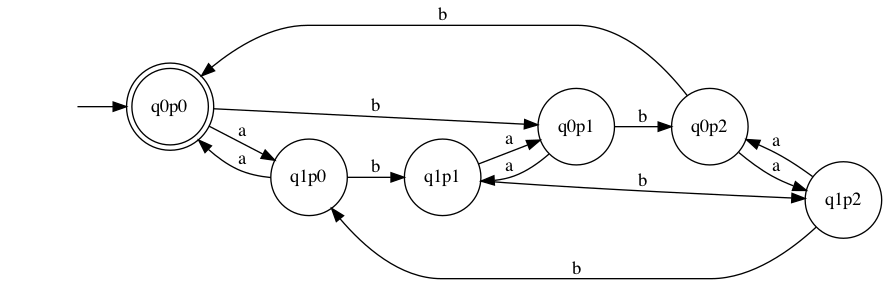
\includegraphics[width=0.8\textwidth]{g23.png}
    \end{center}


%%%%%%%%%%%%%%% 2.4 %%%%%%%%%%%%%%%
\item {$L_4 = \overline{L_3}$\\} \\ \\
    \text{Конечные вершины} \longleftrightarrow \text{начальные вершины}
    \begin{center}
        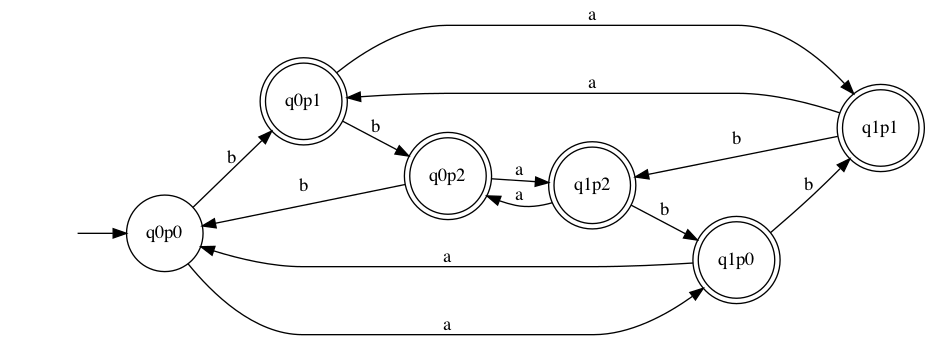
\includegraphics[width=0.8\textwidth]{g24.png}
    \end{center}

%%%%%%%%%%%%%%% 2.5 %%%%%%%%%%%%%%%
5. $L_5 = L_2 \setminus L_3 = L_2 \times L_4 $ \\ \\
    \begin{center}
        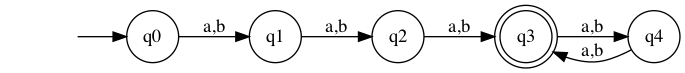
\includegraphics[width=0.8\textwidth]{g251.png}
        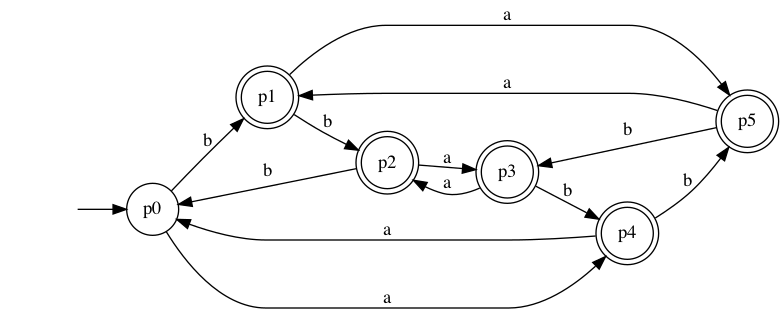
\includegraphics[width=0.8\textwidth]{g252.png}
    \end{center}
    
    \begin{center}
    \[
        \sum = \{a, b\} \\
        S = \left\langle q0,p0 \right\rangle \\
        T = \{q3p1, q3p2, q3p3, q3p4, q3p5\}
    \]
    \end{center}
    \begin{center}
        \begin{tabular}{ |c|c|c| } 
        \hline
        $\textbf{qp}$ & $\textbf{a}$ & $\textbf{b}$ \\
        \hline
        00 & 14 & 11\\
        \hline
        01 & 15 & 12\\
        \hline
        02 & 13 & 10\\
        \hline
        03 & 12 & 14\\
        \hline
        04 & 10 & 15\\
        \hline
        05 & 11 & 13\\
        \hline\hline
        10 & 24 & 21\\
        \hline
        11 & 25 & 22\\
        \hline
        12 & 23 & 20\\
        \hline
        13 & 22 & 24\\
        \hline
        14 & 20 & 25\\
        \hline
        15 & 21 & 23\\
        \hline\hline
        20 & 34 & 31\\
        \hline
        21 & 35 & 32\\
        \hline
        22 & 33 & 30\\
        \hline
        23 & 32 & 34\\
        \hline
        24 & 30 & 35\\
        \hline
        25 & 31 & 33\\
        \hline\hline
        30 & 44 & 41\\
        \hline
        31 & 45 & 42\\
        \hline
        32 & 43 & 40\\
        \hline
        33 & 42 & 44\\
        \hline
        34 & 30 & 45\\
        \hline
        35 & 41 & 43\\
        \hline\hline
        40 & 34 & 51\\
        \hline
        41 & 35 & 32\\
        \hline
        42 & 33 & 30\\
        \hline
        43 & 32 & 34\\
        \hline
        44 & 30 & 35\\
        \hline
        45 & 31 & 33\\
        \hline
        \end{tabular}
    \end{center} 
            
    \begin{center}
        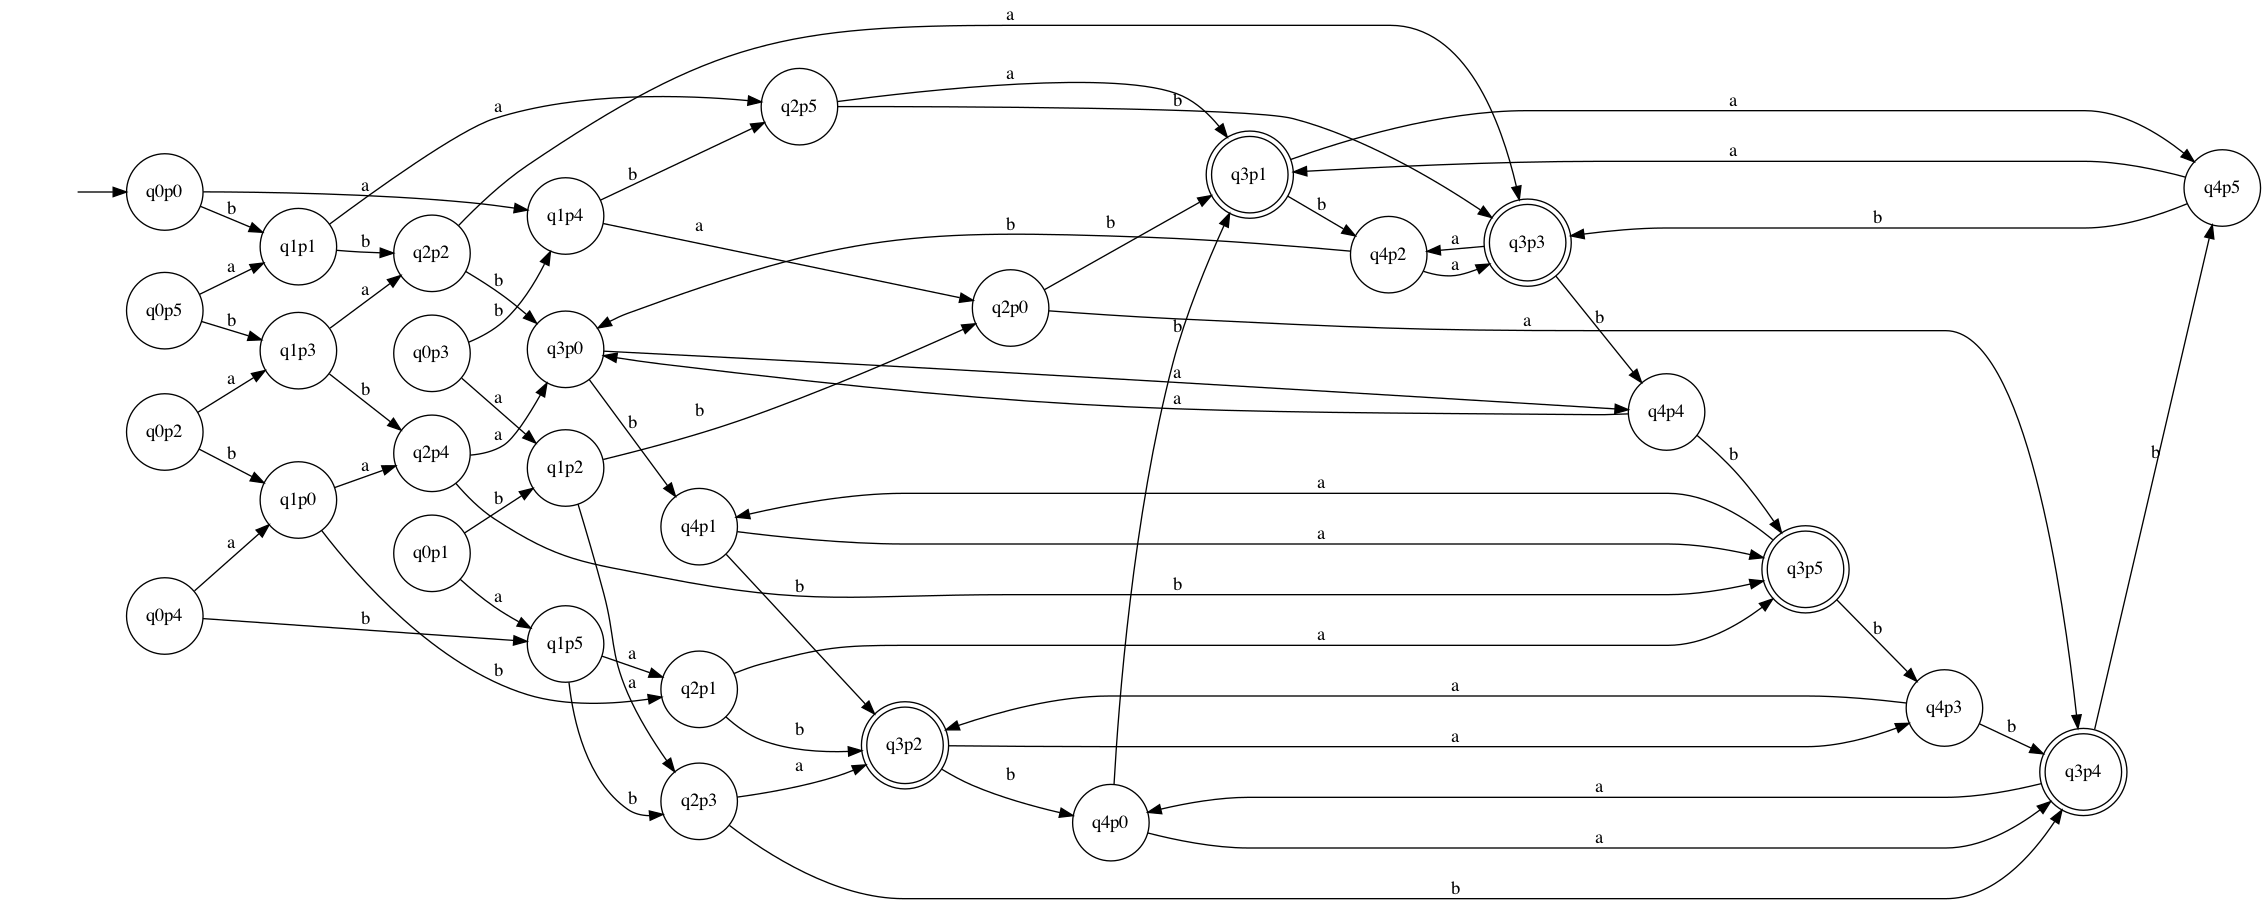
\includegraphics[width=1.1\textwidth]{g25.png}
    \end{center}
\end{enumerate}







%%%%%%%%%%%%%%%%%%%%%%%%%%%%%%%%%%%%%%%%%%% Задание 3 %%%%%%%%%%%%%%%%%%%%%%%%%%%%%%%%%%%%%%%%%%%
\section{Задание №3. Построить минимальный ДКА по регулярному выражению.}

\begin{enumerate}

%%%%%%%%%%%%%%% 3.1 %%%%%%%%%%%%%%%
\\
\item {$ (a b +a b a)^*a $} \\ \\
    НКА с $\lambda$-переходами:
    \begin{center}
        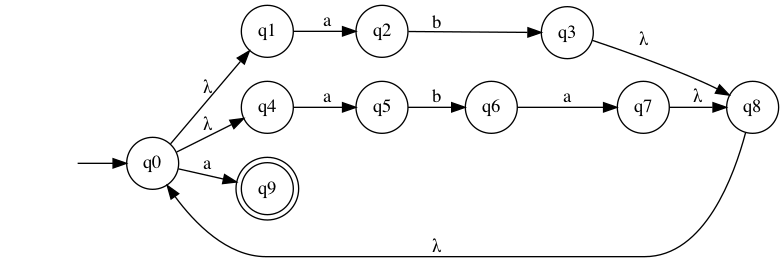
\includegraphics[width=0.8\textwidth]{g31_nka.png}
    \end{center}
    
    \begin{center}
        \begin{tabular}{|c|c|c|}
            \hline
            \textbf{Q} & \textbf{a} & \textbf{b} \\
            \hline
            q0 & q2 q5 q9 & - \\
            \hline
            q2 q5 q9 & - & q3 q6 \\
            \hline
            q3 q6 & q2 q5 q7 q9 & - \\
            \hline
            q2 q5 q7 q9 & q2 q5 q9 & q3 q6 \\
            \hline
        \end{tabular}\\
    \end{center}
    
    МДКА:
    \begin{center}
        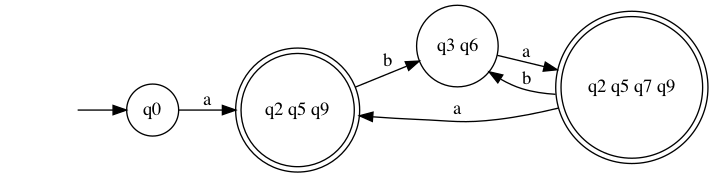
\includegraphics[width=0.8\textwidth]{g31.png} \\
    \end{center}

%%%%%%%%%%%%%%% 3.2 %%%%%%%%%%%%%%%
\item {$ a(a(ab)^*b)^*(ab)^* $} \\ \\
    НКА с $\lambda$-переходами:
    \begin{center}
        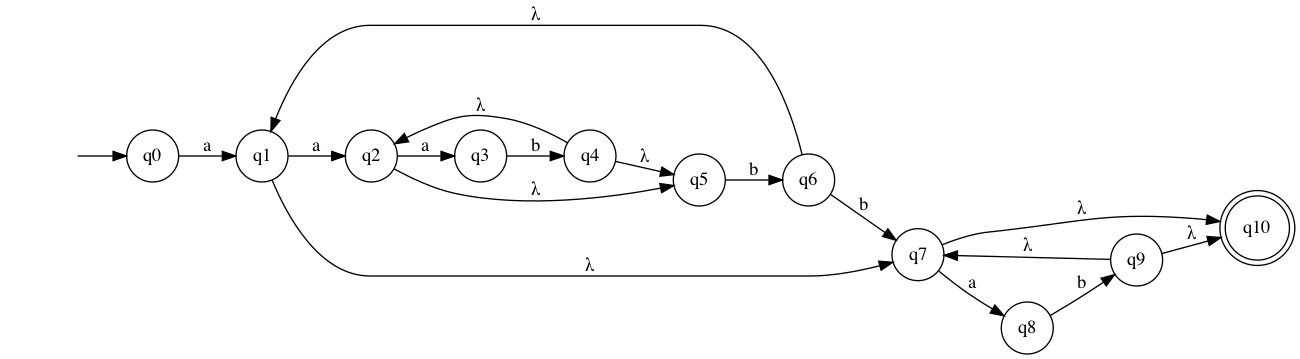
\includegraphics[width=1\textwidth]{g32_nka.png}
    \end{center}
    
    ДКА без $\lambda$-переходов:
    \begin{center}
        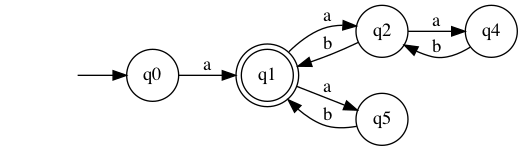
\includegraphics[width=0.5\textwidth]{g32_dka.png}
    \end{center}
    
    МДКА:
    \begin{center}
        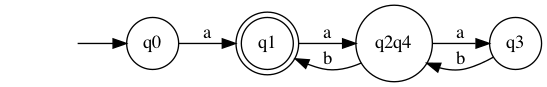
\includegraphics[width=0.5\textwidth]{g32_mdka.png}
    \end{center}
    
%%%%%%%%%%%%%%% 3.3 %%%%%%%%%%%%%%%
\item {$ (a + (a + b)\textbf{(}a + b)b\textbf{)}^* $} \\ \\
    НКА без $\lambda$-переходов:
    \begin{center}
        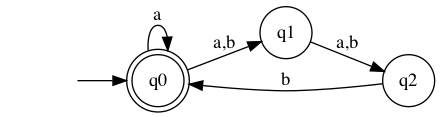
\includegraphics[width=0.5\textwidth]{g33_nka.png}
    \end{center}
    
    \begin{center}
        \begin{tabular}{|c|c|c|}
            \hline
            \textbf{Q} & \textbf{a} & \textbf{b} \\
                \hline
                q0 & q0 q1 & q1 \\
                \hline
                q0 q1 & q0 q1 q2 & q1 q2 \\
                \hline
                q0 q1 q2 & q0 q1 q2 & q0 q1 q2 \\
                \hline
                q1 & q2 & q2 \\
                \hline
                q1 q2 & q2 & q0 q2 \\
                \hline
                q2 & - & q0 \\
                \hline
                q0 q2 & q0 q1 & q0 q1 \\
                \hline
        \end{tabular}\\
    \end{center}
    МДКА:
    \begin{center}
        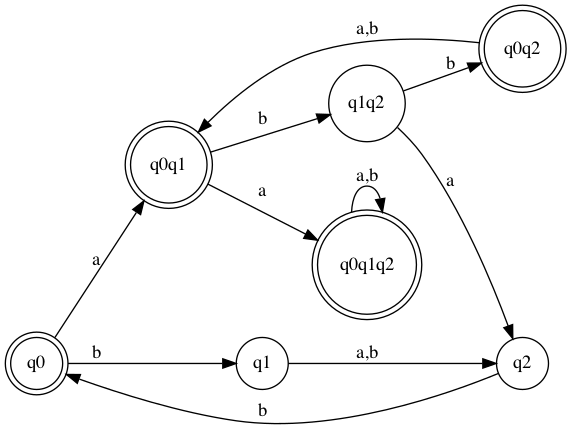
\includegraphics[width=0.5\textwidth]{g33.png}
    \end{center}
    
%%%%%%%%%%%%%%% 3.4 %%%%%%%%%%%%%%%
\item {$ (b + c)((ab)^* c + (b a)^*)^* $} \\ \\
    НКА с $\lambda$-переходами:
    \begin{center}
        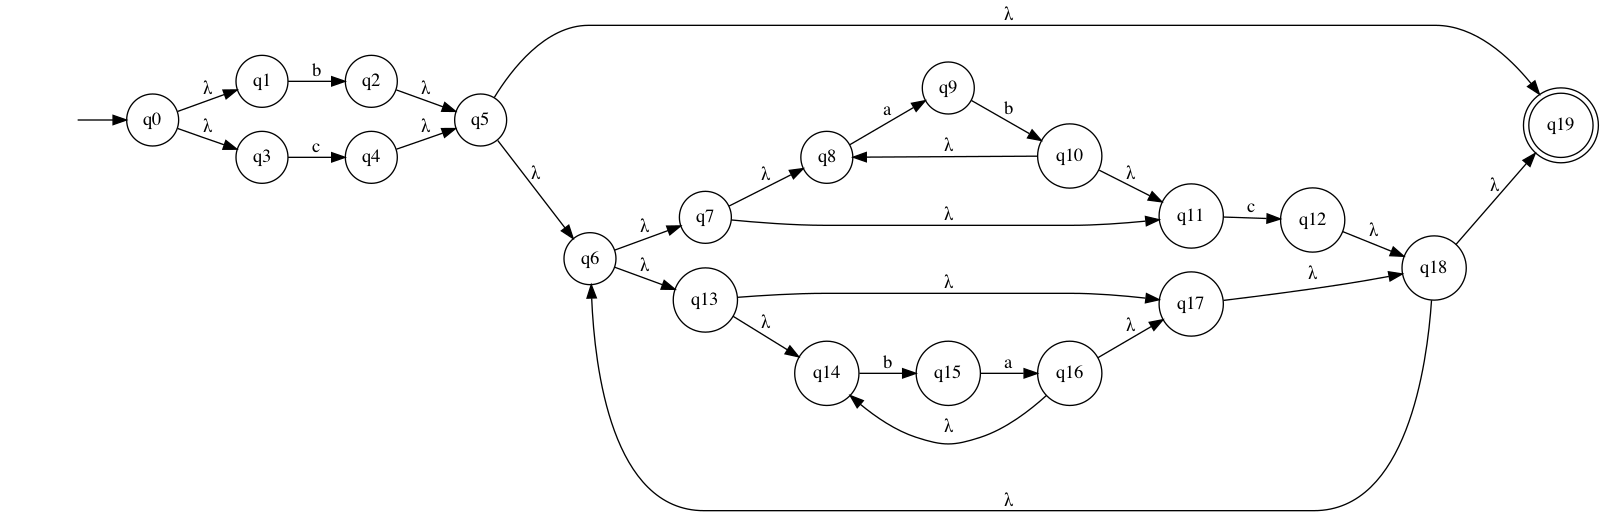
\includegraphics[width=1\textwidth]{g34_nka.png}
    \end{center}
    
    
    ДКА без $\lambda$-переходов:
    \begin{center}
        \begin{tabular}{|c|c|c|c|}
            \hline
            \textbf{Q} & \textbf{a} & \textbf{b}& \textbf{с}  \\
            \hline
            {0,1,3} & - & {2,5,6,7,8,11,13,14,17,18,19} & {4,5,6,7,8,11,13,14,17,18,19} \\
            \hline
            {2,5,6,7,8,11,13,14,17,18,19} & {9} & {15} & {6,7,8,11,12,13,14,17,18,19} \\
            \hline
            {4,5,6,7,8,11,13,14,17,18,19} & {9} & {15} & {6,7,8,11,12,13,14,17,18,19} \\
            \hline
            {9} & {-} & {8,10,11} & {-} \\
            \hline
            {15} & {6,7,8,11,12,13,14,17,18,19} & {-} & {-} \\
            \hline
            {6,7,8,11,12,13,14,17,18,19} & {9} & {15} & {6,7,8,11,12,13,14,17,18,19} \\
            \hline
            {8,10,11} & {9} & {-} & {6,7,8,11,12,13,14,17,18,19} \\
            \hline
            {6,7,8,11,12,13,14,17,18,19} & {9} & {15} & {6,7,8,11,12,13,14,17,18,19} \\
            \hline
        \end{tabular}\\
    \end{center}
    
    Введём обозначения для простоты восприятия
    \begin{center}
        \begin{tabular}{|c|c|c|c|}
        \hline
        \textbf{A} & \textbf{B} & \textbf{C}& \textbf{D}& 
        \hline
        \{0,1,3\}&
        \{2,5,6,7,8,11,13,14,17,18,19\}&
        \{4,5,6,7,8,11,13,14,17,18,19\}&
        \{9\}&
        \hline
        \end{tabular} \\
    \end{center}
    \begin{center}
        \begin{tabular}{|c|c|c|c|}
        \hline
        \textbf{E} & \textbf{F} & \textbf{G}& \textbf{H}&
        \hline
        \{15\}&
        \{6,7,8,11,12,13,14,17,18,19\}&
        \{8,10,11\}&
        \{6,7,8,11,12,13,14,17,18,19\} \\
        \hline
        \end{tabular} \\
    \end{center}
    \begin{center}
        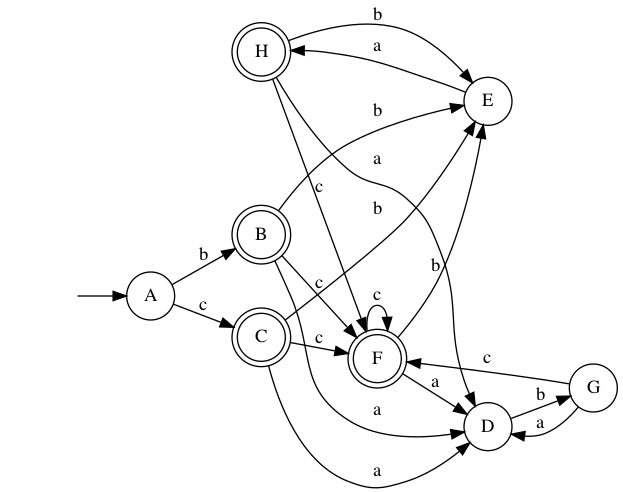
\includegraphics[width=0.8\textwidth]{g34_dka.png}
    \end{center}
    \begin{center}
        \begin{tabular}{|c|c|c|c|c|}
        \hline
        \textbf{p0} & \textbf{p1} & \textbf{p2}& \textbf{p3}& \textbf{p4} \\
        \hline
        \{A\}&
        \{B,C,F,H\}&
        \{D\}&
        \{E\}&
        \{G\}&
        \hline
        \end{tabular} \\
    \end{center}
    
    \newpage
    МДКА:
    \begin{center}
        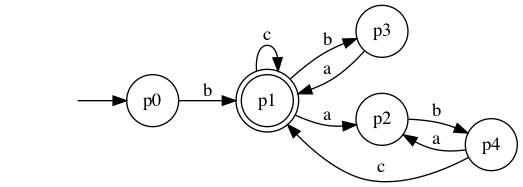
\includegraphics[width=0.7\textwidth]{g34_mdka.png}
    \end{center}

%%%%%%%%%%%%%%% 3.5 %%%%%%%%%%%%%%%
\item {$ (a + b)^+(a a + b b + a b a b + b a b a)(a + b)^+ $} \\ \\
    НКА без $\lambda$-переходов:
    \begin{center}
        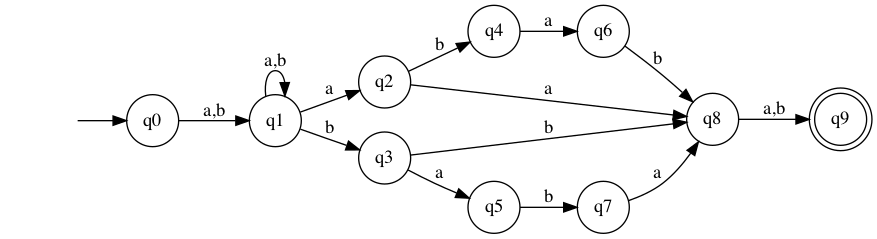
\includegraphics[width=0.9\textwidth]{g35_nka.png}
    \end{center}
    Не осилил такой большой граф

\end{enumerate}


%%%%%%%%%%%%%%%%%%%%%%%%%%%%%%%%%%%%%%%%%%% Задание 4 %%%%%%%%%%%%%%%%%%%%%%%%%%%%%%%%%%%%%%%%%%%
\section{Задание №4. Определить является ли язык регулярным или нет.}
 
\begin{enumerate}
    \item {$ L = \{(a a b)^{n} b(a b a)^{m} \mid n \ge 0, m \ge 0 \}$} \\
        \begin{center}
            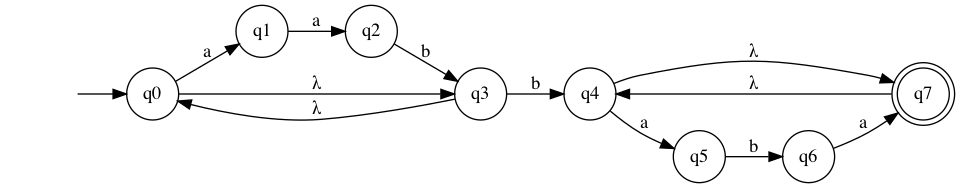
\includegraphics[width=1\textwidth]{g41.png}
        \end{center}
        \textbf{Язык регулярный, построен конечный автомат.} \\

    \item {$L = \{{u a a v \mid u \in \{a, b\}^*, v \in \{a, b\}^*, |u|_b \ge |v|_a}\} $}\\ \\
        Для доказательства нерегулярности удобно использовать отрицание леммы о накачке. \\
        Возьмём (зафксируем) $n$. \\
        Рассмотрим слово $w = b^naaa^n, \quad |w| = 2n+2 \geq  n$. \\
        Представим слово $w$ в виде разбиения $w=xyz$, так что $|xy| \leq n$, $|y| > 0$. \\
        $x = b^i, \quad y = b^j,  \quad i+j \leq n, \quad j > 0, \quad z = b^{n-i-j}aaa^n$ \\
        Тогда слово $\quad x y^0 z = b^i (b^j)^0 b^{n-i-j} a a a^n = b^{n-i} a a a^n \notin L$ \\ \\
        \textbf{Язык не является регулярным.} \\
        
   \item {$L = \{ a^mw \ \mid \ w \in \{ a,b \}^*, 1 \leq |w|_b \leq m \}$} \\ \\
        $w = a^n b^n , |w| \geq n$ \\
        $w = xyz, |xy| \leq n$, $|y| > 0$ \\
        $x = a^i, \quad y = a^j, \quad i+j \leq n, \quad j > 0, \quad z = a^{n-i-j}b^n$ \\
        Тогда слово $\quad x y^0 z = a^i (a^j)^0 a^{n-i-j} b^n = a^{n-i} b^n \notin L$ \\ \\
        \textbf{Язык не является регулярным.} \\
        
    \item {$L = \{ a^k b^m a^n \mid k = n \lor m > 0\} $}\\ \\
        $w = a^nba^n, w \geq n$ \\
        $w = xyz, \quad |xy| \leq n, \quad |y| > 0$ \\
        $x = a^i, \quad y = a^j, \quad i+j \leq n, \quad j > 0, \quad z = a^{n-i-j} b a^n$ \\
        Тогда слово $\quad x y^k z = a^i a^{jk} a^{n-i-j} b a^n = a^{n-j(k-1)} b a^n \notin L \quad \forall k > 1$ \\ \\
        \textbf{Язык не является регулярным.} \\
        
    \item {$L = \{ucv \mid u \in \{a, b\}^*, v \in \{a, b\}^*, u \neq v^R\} $}\\ \\
        $w = (ab)^n c (ba)^n, w \geq n$ \\
        $w = xyz, \quad |xy| \leq n, \quad |y| > 0$ \\
        $x = \alpha_1\alpha_2...\alpha_i, \quad y=\alpha_{i+1}\alpha_{i+2}...\alpha_{i+j}, \quad i+j \leq n, \quad j > 0, \quad z = \alpha_{i+j+1}\alpha_{i+j+2}...\alpha_{2n} c (ba)^n$ \\
        Тогда слово $\quad x y^k z = \alpha_1...\alpha_i(\alpha_{i+1}...\alpha_{i+j})^k \alpha_{i+j+1}...\alpha_{2n}c(ba)^n \notin L \quad \forall k > 0 $ \\ \\
        \textbf{Язык не является регулярным.} \\
        
        
\end{enumerate}

\end{document}
